\chapter{Simulation Monte Carlo}
    \section{Introduction}
        Les chapitres précédents ont permis à l'étudiant·e de se familiariser avec la simulation de systèmes déterministes, c'est-à-dire de systèmes dans lesquels le comportement peut être univoquement prédit en connaissant les conditions initiales. Dans le cas contraire, le système est dit \textit{stochastique}. De tels systèmes requièrent de nouveaux outils pour étudier leur comportement. Nous présentons une telle méthode, appelée \textit{simulation Monte Carlo}.
        
        Une simulation de Monte Carlo est une méthode statistique utilisée pour estimer le comportement d'un système complexe en modélisant l'incertitude de ses paramètres grâce à des tirages aléatoires. En répétant de nombreuses fois des simulations qui incluent des éléments de hasard, elle permet d'obtenir une approximation de l'impact de ces incertitudes sur les résultats. 
        
        La modélisation du système commence par la définition d'un modèle du problème à étudier, en identifiant les variables et les paramètres d'intérêt. Ensuite, les incertitudes sont représentées par des distributions de probabilité. Par exemple, si un temps avant un évènement varie, cette variation peut être modélisée par une distribution normale, exponentielle, ou autre. Pour chaque simulation, des tirages aléatoires sont effectués pour chaque paramètre incertain, en suivant la distribution définie. En utilisant les valeurs tirées, on simule le comportement du système et on enregistre les résultats. Ce processus est répété un grand nombre de fois afin de capturer un large échantillon de scénarios possibles. Finalement, une analyse statistique est effectuée sur les résultats des simulations pour estimer des métriques telles que la moyenne, l'écart-type, la distribution des résultats, ou des intervalles de confiance.

    \section{Générateur uniforme}
        Nous rappellerons quelques définitions essentielles pour la compréhension de cette section. Cependant, nous référons l'étudiant·e au cours de Probabilités et Statistique (\cite{mathf315_1, mathf315_2}) pour un aperçu plus extensif des notions utiles.

        Le syllabus offre une explication extensive de la nécessité degénérateur de nombres uniformes (\cite{infof305}). Dans cette section, nous proposons des implémentations pour les méthodes expliquées dans le syllabus.
        \subsection{Méthode de Neumann}
            John von Neumann\footnote{John von Neumann était un mathématicien américano-hongrois né en 1903 et décédé en 1957. Ses contributions vont de la mécanique quantique à l'informatique théorique en passant par les sciences économiques. Son intérêt pour le développement de la méthode Monte Carlo date de la période de la Seconde Guerre Mondiale. Il a notamment participé au projet Manhattan.} a proposé, en étudiant les simulations Monte Carlo, qui nécessitaient bien entendu une méthode pour générer des nombres pseudo-aléatoires, la méthode qui a donné son nom(\cite{von195113}). Le code suivant en montre une implémentation.
            \inputminted{python}{codes/von_neumann.py}
            Cependant, lorsque le système atteint l'état $0$, il reste bloqué, c'est un état absorbant. 
            
        \subsection{Générateur congruentiel linéaire}
            Rapidement après la méthode proposée par von Neumann, Lehmer\footnote{Derrick Lehmer était un mathématicien américain né en 1905 et décédé en 1991. Ses contributions concernent principalement des problèmes d'analyse et de théorie des nombres, pour lesquel il fut un pionnier dans l'utilisation d'ordinateurs et de méthodes numériques. Notamment, il travailla avec sa femme Emma Markovna Trotskaya comme opérateur sur l'ENIAC, le premier ordinateur Turing-complet entièrement éléctronique.} proposa un autre algorithme pour la génération de nombre suivant une distribution pseudo-aléatoire uniforme (\cite{lehmer1951}). Nous en montrons une implementation dans le code suivant.
            \inputminted{python}{codes/LGC.py}
            
        \subsection{Test de \textit{randomness}}
            Afin de vérifier si les générateurs de nombres pseudo-aléatoires que nous avons présentés sont fiables, en pratique, il est possible de réaliser des tests statistiques comparant la distribution des échantillons qu'ils produisent avec la distribution uniforme. Nous en présentons quelques implémentations.
            \subsubsection{Test des moments}
                \begin{definition}{Moment brut}
                    Soit un échantillon $x_1, x_2, ..., x_n$ de réalisations d'une variable aléatoire $\mathbf{X}$. Le $n^{\text{ème}}, n \in \mathbb{N_0^+}$ \textbf{moment brut} autour de l'origine de $\mathbf{X}$ est donné par
                    \begin{equation}
                        \mathbb{E}(\mathbf{X}^n) = \int_{-\infty}^{+\infty} x^n f(x) \, dx
                    \end{equation}
                    
                    Sa valeur peut être estimé par la fonction
                    \begin{equation}
                        \hat{m}_k = \frac1n \sum_{i=0}^n x_i^k
                    \end{equation}
                \end{definition}
                Ainsi, on peut vérifier si les générateurs proposés pour la distribution uniforme sur $[0, 1]$ respectent les moments attendus. Le code suivant montre que le générateur congruentiel linéaire vérifie ce test.
                \inputminted{python}{codes/moments_test.py}

            \subsubsection{Test $\chi^2$}
                Si l'on divise l'intervalle $[0, 1]$ en $s$ sous-intervalles de taille égale, et que l'échantillon de taille $N$ que l'on étudie respecte une distribution uniforme, alors, chaque sous-intervalle devrait contenir, en moyenne, $s/N$ éléments. Soit $c_j$ le nombre mesuré d'éléments dans le sous-intervalle $j$. On peut quantifier la quantité
                \begin{equation}
                    C = \frac{s}{N} \sum_{j=1}^s (c_j - \frac{N}{s})^2
                \end{equation}
                qui est une mesure de la concordance entre le nombre d'éléments attendus et le nombre d'éléments mesurés. 

                Si l'échantillon respectent une distribution uniforme, alors la quantité $C$ est distribuée comme une variable $\chi^2$ à $s-1$ degrés de liberté (on réfèrera l'étudiant·e au cours de statistiques (\cite{mathf315_2})). Le module \codeword{scipy.stats} propose une classe \codeword{chi2}. La méthode \codeword{cdf(aC, s)} de cette classe permet d'obtenir la p-value, c'est-à-dire la probabilité sous l'hypothèse nulle d'observer une valeur aussi extrême que celle obtenue. L'hypothèse nulle décrite ici est l'hypothèse d'uniformité. Si cette p-value est en-dessous d'un seuil critique choisi (typiquement, 5\%), alors on rejette l'hypothèse nulle, parce qu'il est très peu probable qu'en vérifiant l'hypothèse on obtienne la valeur observée. Un exemple est donné dans le code suivant.
                \inputminted{python}{codes/chi2_test.py}

            \subsubsection{Goodness of fit}
                \begin{definition}{Fonction de répartition empirique}
                    Soit un échantillon $x_1, x_2, ..., x_N$ \textbf{fonction de répartition empirique} est donnée par
                    \begin{equation}
                        \hat{F}_{\mathbf{X}}(x) = \frac{\#x_i < x}{N}
                    \end{equation}
                \end{definition}

                Intuitivement, le test de Kolmogorov-Smirnov compare cette fonction de répartition empirique avec la fonction de répartition théorique en donnant comme estimation le plus grand écart entre ces deux fonctions. La fonction de répartition d'une distribution uniforme est donnée dans le module \codeword{scipy.stats}, mais l'on laissera l'implémentation complète à l'étudiant·e. Le même module offre une fonction macro \codeword{kstest}. On montre dans le code suivant comment vérifier l'uniformité grâce à ce test.
                \inputminted{python}{codes/goodness_of_fit.py}
            
    \section{Générateur aléatoire}
        Le syllabus démontre déjà comment obtenir certaines distribution en modifiant un échantillon d'une distribution uniforme. Nous renvoyons l'étudiant·e vers la démonstration de la méthode de la transformation inverse, pour les distributions uniforme sur un autre intervalle que $[0, 1]$ et pour une distribution exponentielle. Cependant, nous rappelons le fonctionnement de la méthode de la transformation inverse ainsi que de la méthode de rejet.

        \subsection{Méthode de la transformation inverse}
            Soit $\mathbf{X}$ une variable aléatoire avec une fonction de répartition monotone non-décroissante $F_{\mathbf{X}}(x)$. Le syllabus montre en quoi la variable $\mathbf{Y} = F_{\mathbf{X}}(x)$ est toujours distribuée uniformément sur $[0, 1]$. Autrement dit, si l'on sait échantillonner une distribution uniforme sur $[0, 1]$ (ce qui a déjà été montré), on peut utiliser l'inverse de cette fonction de répartition pour obtenir un échantillon suivant la densité $p_{\mathbf{X}}(x)$.

            Par exemple, soit $\mathbf{X}$ une variable aléatoire distribuée uniformément sur l'intervalle $[-1, 1]$. La fonction de répartition de cette variable aléatoire est donnée par
            \begin{equation}
                F_{\mathbf{X}(x- = \frac{x-(-1)}{1-(-1)} = \frac{x+1}{2}}
            \end{equation}
            Soit $u$ un échantillon d'une variable aléatoire uniforme sur $[0, 1]$, alors, par la méthode inverse, on a
            \begin{equation}
                u = \frac{x+1}{2} \Leftrightarrow x = 2u - 1
            \end{equation}
            Donc, si l'on a échantillonné les valeurs suivantes par une méthode de génération pseudo-aléatoire comme présentée précédemment: $[0.423, 0.283, 0.913, 0.559, 0.925]$, la méthode de la transformation inverse les projette sur $[-0.154, -0.434,  0.826,  0.118,  0.85]$. Le script suivant génère $1000000$ valeurs échantillonnées dans une distribution uniforme sur $[0, 1]$, utilise la méthode de la transformation inverse pour les projeter sur la distribution donnée en exemple précédent, et en affiche l'histogramme, donné en figure \ref{fig:inverse_example}.
            \inputminted{python}{codes/inverse_example.py}
            \begin{figure}[h!]
                \centering
                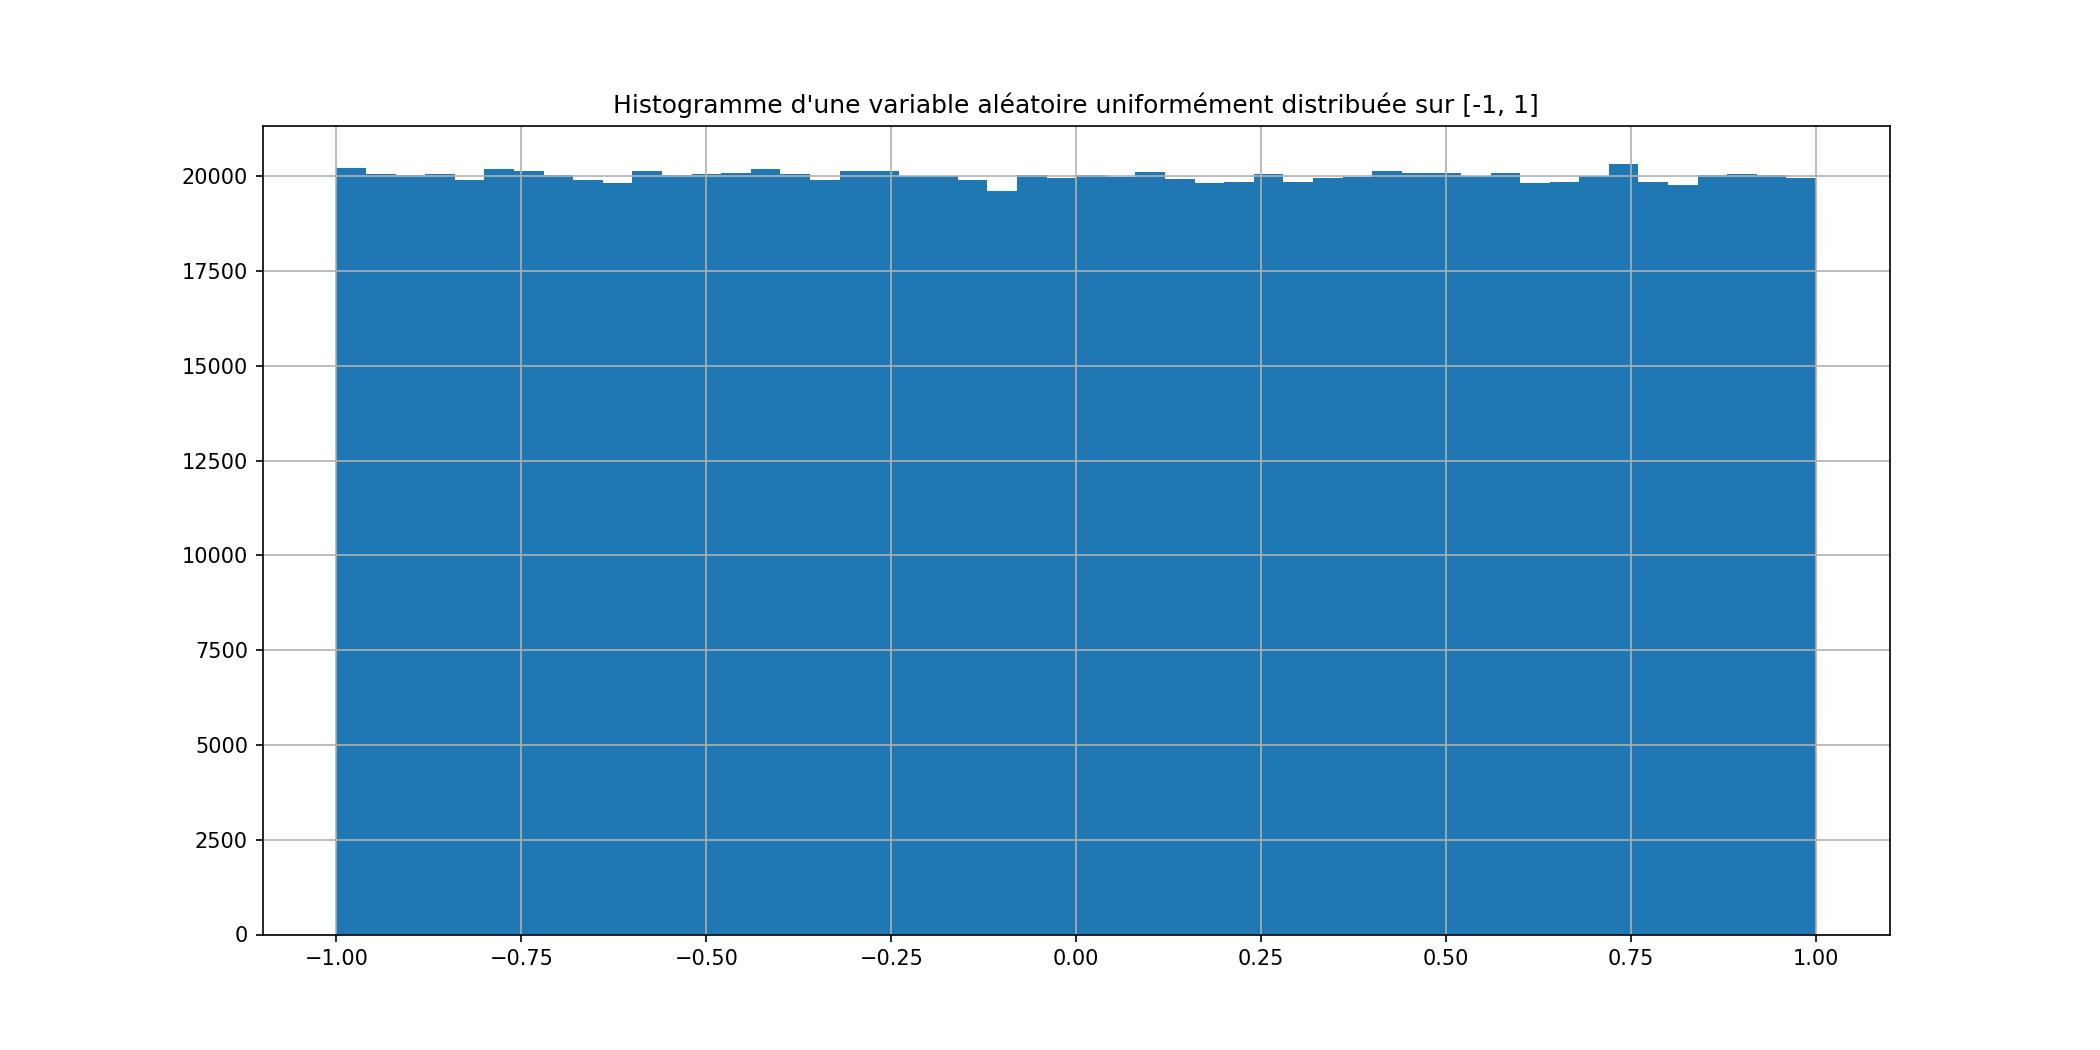
\includegraphics[width=0.8\linewidth]{images/inverse_example.jpg}
                \caption{Histogramme des valeurs obtenue par la méthode de la transformation inverse pour une variable aléatoire uniformément distribuée sur $[-1, 1]$}
                \label{fig:inverse_example}
            \end{figure}

            Le module \codeword{SymPy} propose les fonctions \codeword{solve} et \codeword{lambdify} qui permet, en utilisant du calcul symbolique, d'inverse n'importe quelle fonction de répartition automatiquement (\cite{Simpy2023}). Le code suivant montre comment l'exemple précédent peut être implémenté en \codeword{SymPy}. Le raisonnement utilisé se base sur l'observation que si $f(x) = y \Leftrightarrow f(x) - y = 0$, alors résoudre cette équation pour $x$ donne l'inverse additif de la fonction $f$.
            \inputminted{python}{codes/inverse_lambda.py}
        
        \subsection{Méthode de rejet}
            La méthode de rejet, proposée par von Neumann en 1951, permet d'échantillonner une variable aléatoire qui suit une distribution cible $p_{\mathbf{X}}(x)$.
            Nous voulons échantillonner une telle distribution.
            Admettons que nous ayons un générateur de nombre aléatoire qui échantillonne une distribution suivant une densité $q(x)$. Si il existe un nombre $C>0$ tel que $\forall x, Cq(x) \geq p_{\mathbf{X}}(x)$, autrement dit, que $q(x)$ \textit{est strictement supérieure} en tout point à $p_{\mathbf{X}}(x)$, à un facteur près, alors la méthode de rejet est la suivante:
            \begin{itemize}
                \item Échantillonner une valeur $x$ suivant $q(x)$
                \item Échantillonner une valeur $u$ suivant une distribution indépendante de $q(x)$, typiquement, une distribution uniforme $\mathbf{U}(0, 1)$
                \item Renvoyer $x$ si $u \leq \frac{p_{\mathbf{X}}(x)}{C q(x)}$, sinon, recommencer
            \end{itemize}
            Comment calculer le dernier quotient ? La fonction de densité uniforme est de $1$, et la fonction de densité objective est connue. Donc, dans le cas où l'on choisit $q(x)$ uniforme, le quotient est donné par $\frac{p_{\mathbf{X}}(x)}{C}$.
            
            Il va de soi que ce processus fonctionne si il existe une fonction qui recouvre la densité attendue. Par exemple, les générateurs de distribution uniforme proposés précédemment ne pourraient pas être utilisés pour échantillonner une distribution normale, car sa fonction de densité a une enveloppe infinie (pensez aux queues: comment un rectangle fini pourrait les contenir ?).

    \section{Exercices}
        \subsection{Méthode de rejet}
            \subsubsection{Densité carrée}
                \begin{exercise}{Densité carrée}
                    Écrivez le code python permettant d'échantillonner une distribution décrite par la densité suivante, par la méthode de rejet. Vous pouvez utiliser le générateur uniforme proposé par \codeword{numpy.random}.
                    \begin{equation}
                        p(x) = 
                        \begin{cases}
                            x^2 \text{ si $0\leq x\leq 3^{\frac13}$}\\
                            0 \text{ sinon}
                        \end{cases}
                    \end{equation}
                    Vérifiez analytiquement que la distribution suivant cette densité est correctement normalisée.
                \end{exercise}
                Le code suivant montre la solution. En figure \ref{fig:exercice_rejet_1}, on montre l'histogramme de l'échantillon produit par cette méthode.
                \inputminted{python}{codes/exercice_rejet_1.py}
                \begin{figure}[ht!]
                    \centering
                    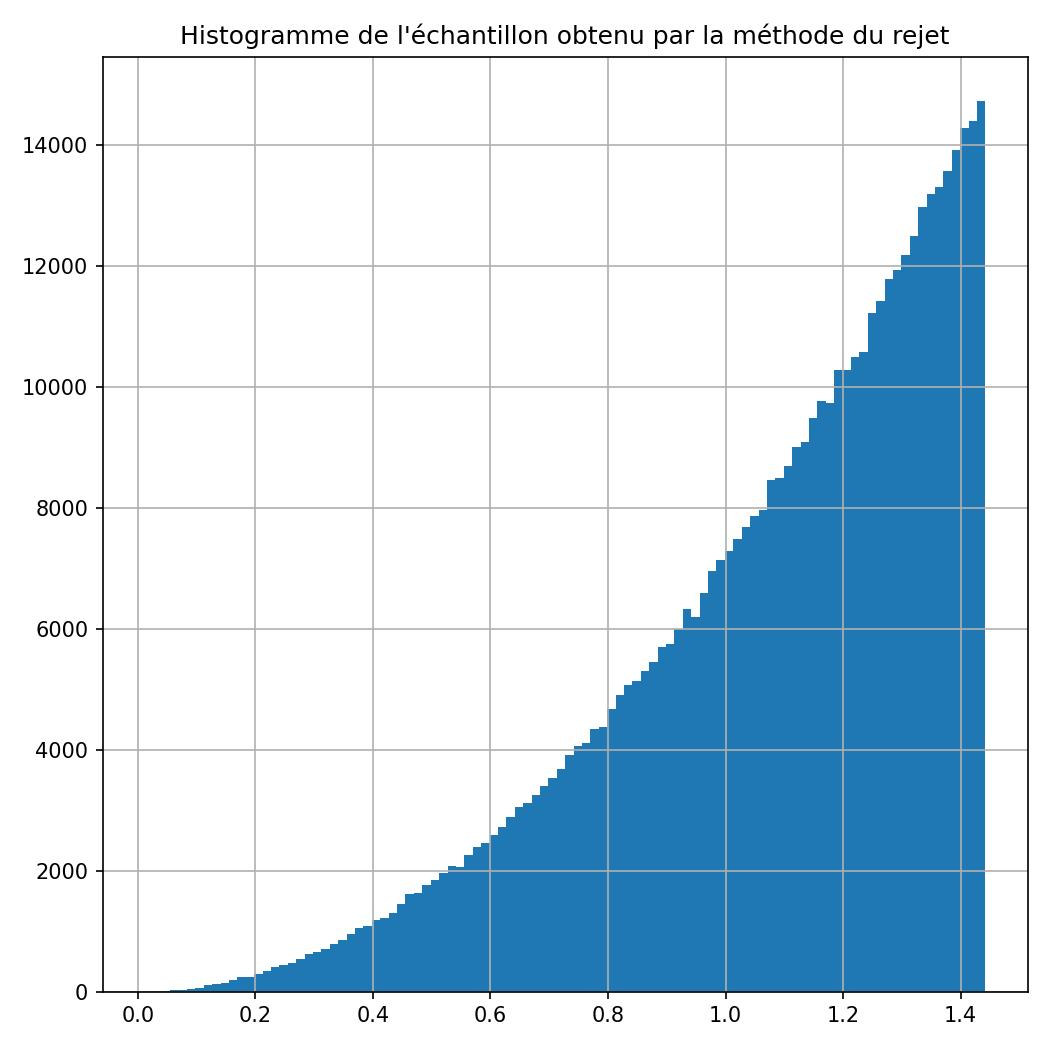
\includegraphics[width=0.7\textwidth]{images/exercice_rejet_1.jpg}
                    \caption{Histogramme de l'échantillon d'une distribution suivant la loi carrée demandée}
                    \label{fig:exercice_rejet_1}
                \end{figure}

            \subsubsection{Densité sinusoïdale}
                \begin{exercise}{Densité carrée}
                    Écrivez le code python permettant d'échantillonner une distribution décrite par la densité suivante, par la méthode de rejet. Vous pouvez utiliser le générateur uniforme proposé par \codeword{numpy.random}.
                    \begin{equation}
                        p(x) = 
                        \begin{cases}
                            \frac{\sin x}{2} \text{ si $0\leq x\leq \pi$ ou si  $2\pi\leq x\leq 3\pi$}\\
                            0 \text{ sinon}
                        \end{cases}
                    \end{equation}
                \end{exercise}
                Le code suivant montre la solution. En figure \ref{fig:exercice_rejet_2}, on montre l'histogramme de l'échantillon produit par cette méthode.
                \inputminted{python}{codes/exercice_rejet_2.py}
                \begin{figure}[ht!]
                    \centering
                    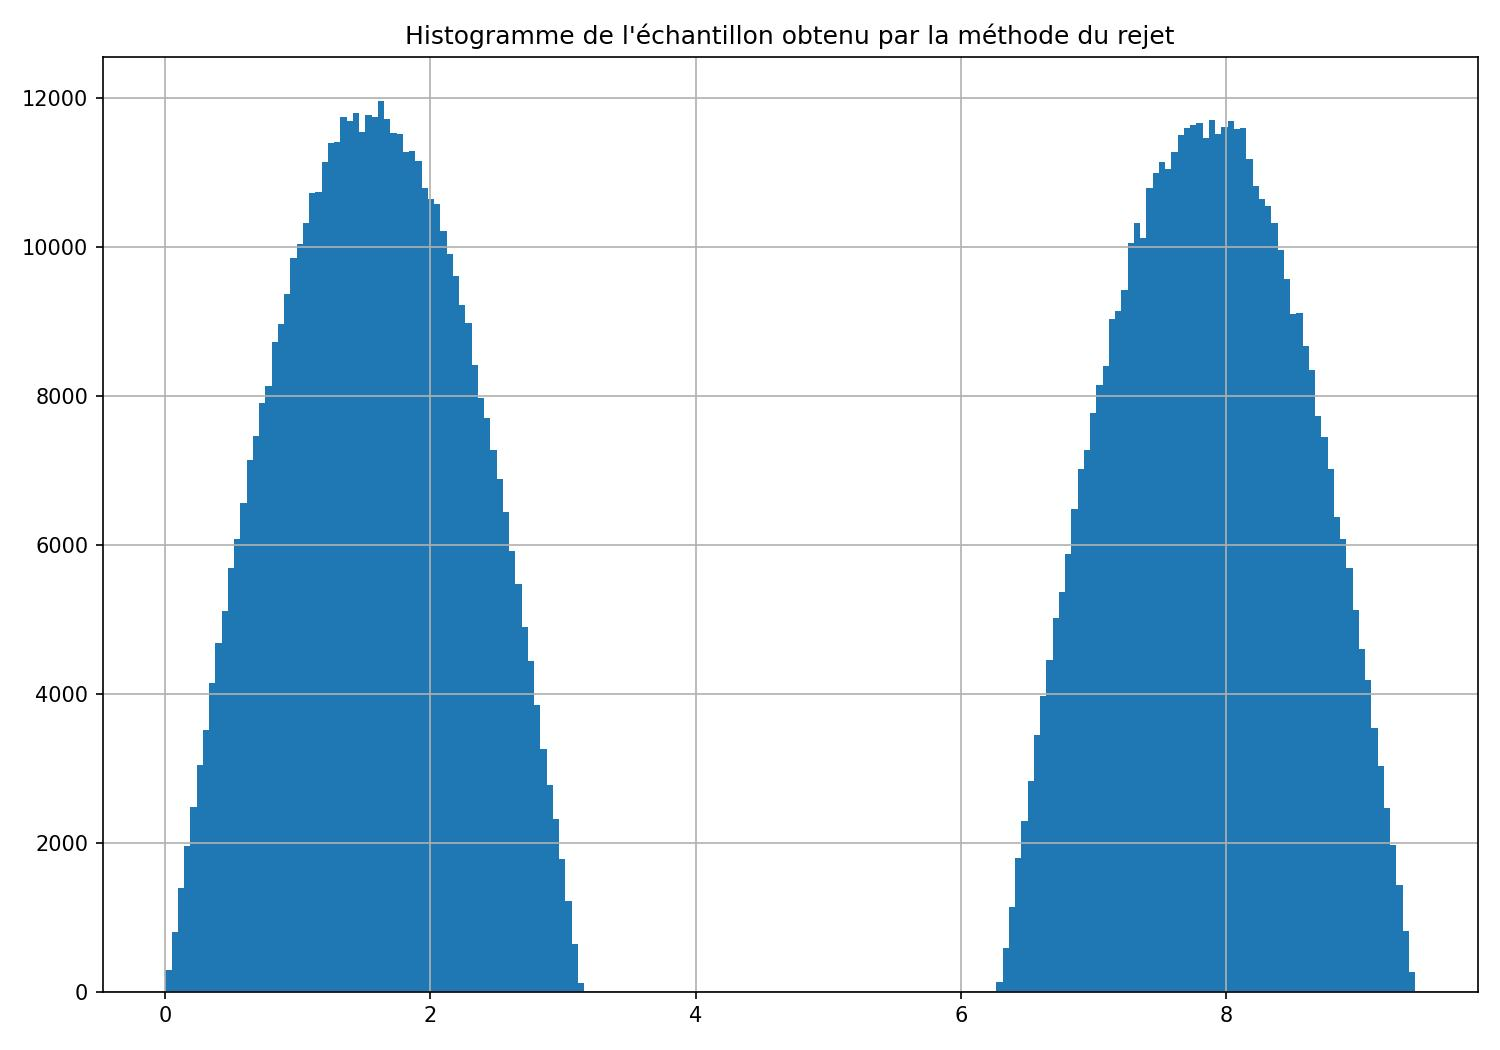
\includegraphics[width=0.7\textwidth]{images/exercice_rejet_2.jpg}
                    \caption{Histogramme de l'échantillon d'une distribution suivant la loi sinusoïdale demandée}
                    \label{fig:exercice_rejet_2}
                \end{figure}

            \subsection{Transformation d'échantillon}
                \begin{exercise}{Transformation d'échantillon}
                    Soit $[0.75, 0.43, 0.39, 0.65, 0.17]$ une série de 5 nombres pseudo-aléatoires générés par un générateur uniforme entre 0 et 1. Utiliser cette série afin de générer par transformation inverse 5 nombres pseudo-aléatoires distribués selon la densité de probabilité
                    \begin{equation}
                        p(x)=
                        \begin{cases}
                            \frac{2}{a}(1-\frac{x}{a})\text{ si $0\leq x\leq a$}\\
                            0 \text{ ailleurs}
                        \end{cases}
                    \end{equation}
                    pour $a=1$ et $a=4$.
                \end{exercise}
                Nous donnons la solution pour $a=1$. La fonction de répartition est donnée par
                \begin{equation}
                    F(x)=
                    \begin{cases}
                        0\text{ si $x<0$}\\
                        2(1-x)x = 2x-x^2\text{ si $0\leq x\leq 1$}\\
                        1 \text{ si $x>1$}
                    \end{cases}
                \end{equation}
                On peut utiliser le script suivant pour calculer les valeurs par la méthode inverse:
                \inputminted{python}{codes/exercice_inverse_1.py}

    \section{Simulation Monte Carlo}
        Les méthodes probabilistes et les simulations de Monte Carlo constituent des outils essentiels en informatique, offrant des solutions efficaces à des problèmes complexes souvent inaccessibles par des approches analytiques classiques. Leur champ d’application est vaste, couvrant notamment la physique statistique, les mathématiques financières, la mécanique quantique, l’apprentissage automatique ou encore la biologie.

        Le cœur de la méthode de Monte Carlo repose sur l’échantillonnage aléatoire pour obtenir des approximations numériques. Plutôt que de chercher une solution exacte par le biais de formules analytiques, ces techniques s’appuient sur la loi des grands nombres pour estimer les résultats via des simulations répétées. Cette approche s’avère particulièrement utile face à des espaces de grande dimension, des géométries complexes ou des systèmes comportant de nombreux degrés de liberté.
        
        Un exemple simple permet d’illustrer ce principe: imaginons que vous souhaitiez estimer la surface d’un lac dont la forme est irrégulière et difficile à modéliser mathématiquement. Vous l’entourez alors d’un carré dont les dimensions sont connues avec précision. En lançant aléatoirement un grand nombre de pierres dans cette zone à l’aide d’une catapulte, vous pouvez observer la proportion de pierres qui tombent dans le lac par rapport au total. Cette proportion est approximativement égale au rapport entre la surface du lac et celle du carré. Plus le nombre de lancers est élevé, plus l’estimation gagne en précision. Ce procédé illustre le fonctionnement de l’intégration par Monte Carlo.
        
        \subsection{Exemple classique}
            \subsubsection{Estimation d'une intégrale définie}
                Tracer une fonction sur un plan n'est pas une tâche difficile. En effet, il suffit d'en calculer la valeur en tous les points du plan. En déterminer l'intégrale, cependant, peut parfois, d'un point de vue analytique, être une tâche plus ardue.
                
                Rappelez-vous, cependant, que la définition d'une intégrale (définie) est formellement l'aire de la surface entre la fonction et l'abscisse. Imaginez maintenant: vous délimitez une certaine surface d'intérêt pour la fonction que vous étudiez, dont vous connaissez la surface (par exemple, un rectangle), autour du tracé de la fonction. Vous échantillonnez aléatoirement des points sur cette surface. Si le nombre de points est suffisamment grand, la proportion de points se trouvant sous la courbe de la fonction correspond à la proportion de l'aire sous cette courbe par rapport à l'aire du rectangle d'échantillonnage. 

                Le code suivant utilise cette méthode pour déterminer la valeur de l'intégrale de la fonction $f(x) = x^2$ entre $0$ et $1$. La figure \ref{fig:montecarlo_integral} montre les points échantillonnés, classés selon leur position par rapport à la courbe de la fonction.
                \inputminted{python}{codes/montecarlo_integral.py}
                \begin{figure}[ht!]
                    \centering
                    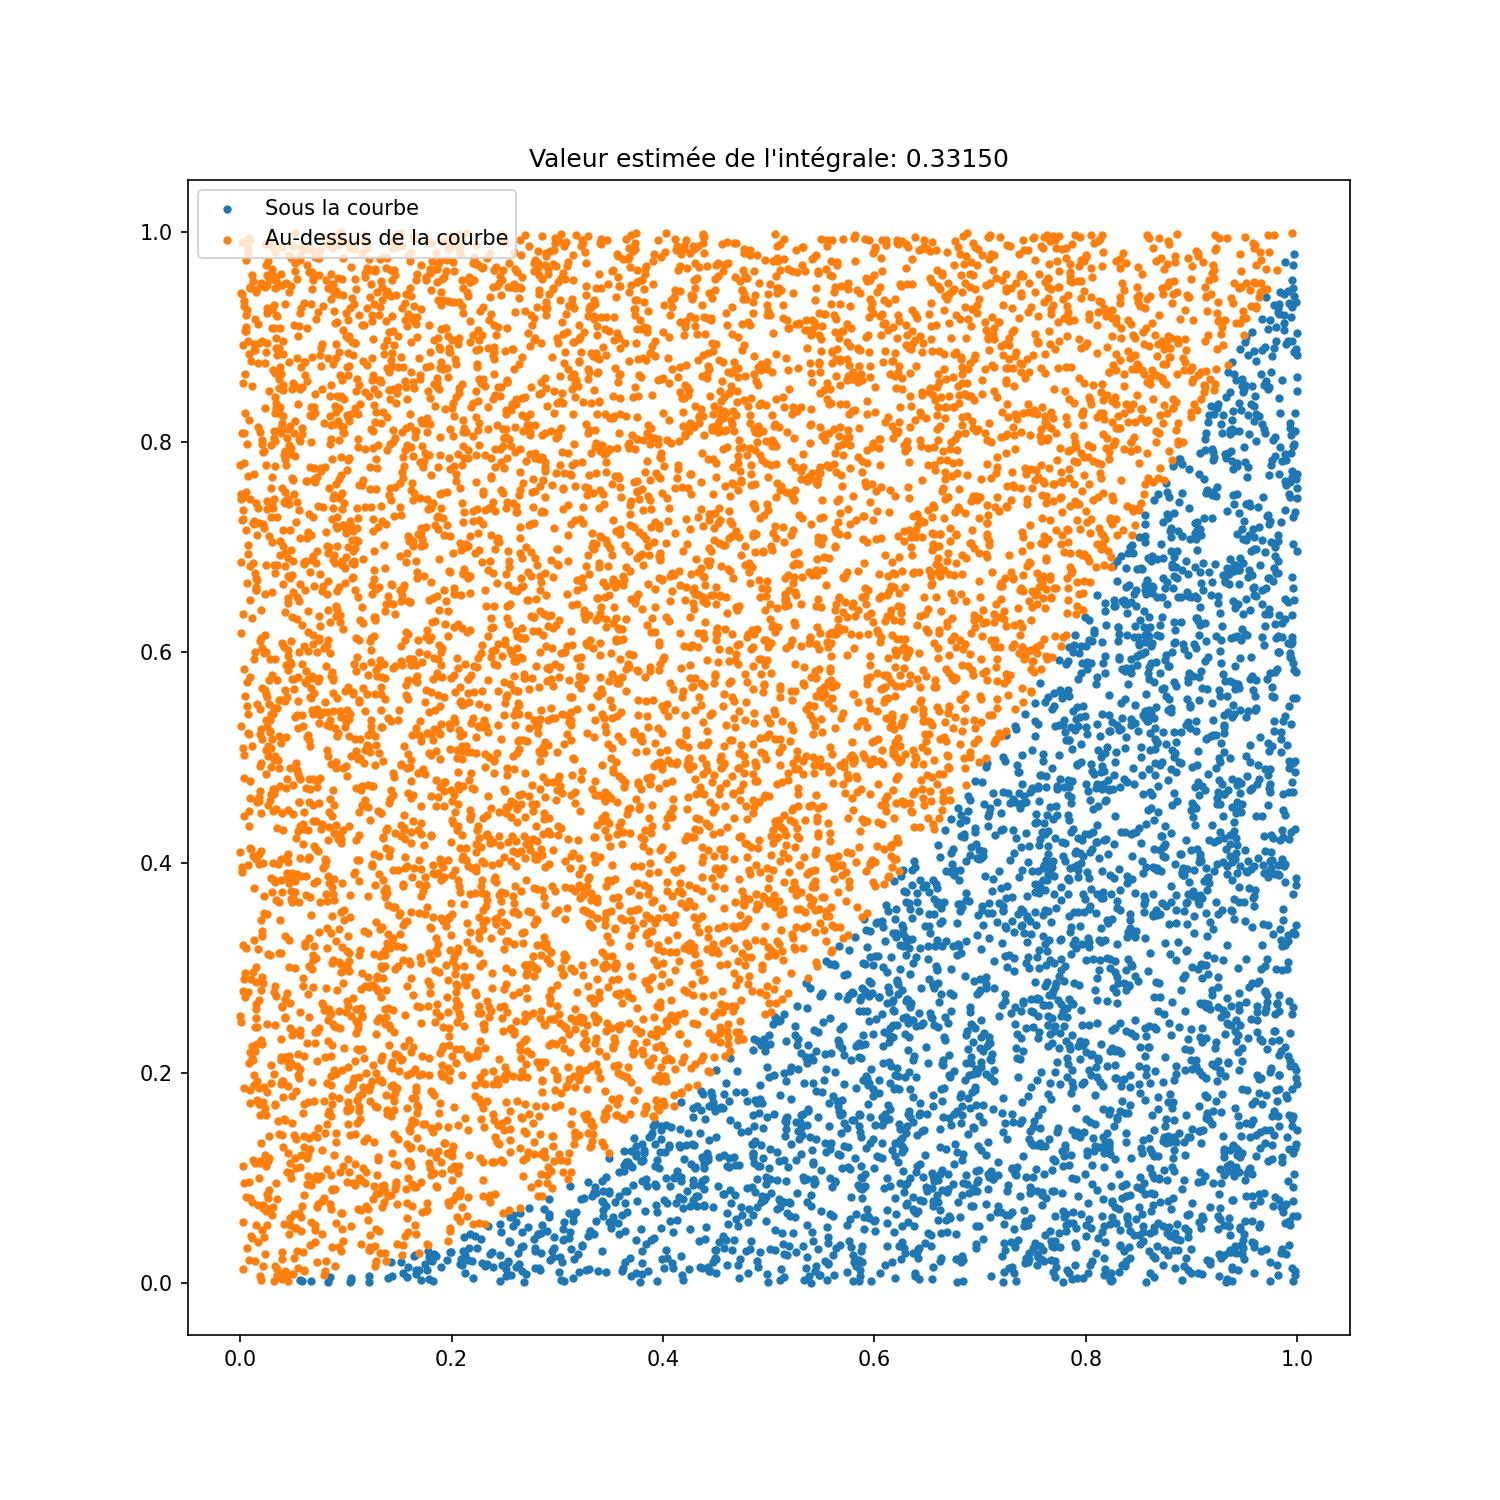
\includegraphics[width=0.7\textwidth]{images/montecarlo_integral.jpg}
                    \caption{Simulation Monte Carlo pour estimer la valeur de l'intégrale de $f(x)=x^2$ sur $[0, 1]$}
                    \label{fig:montecarlo_integral}
                \end{figure}
    
    \section{Exercices}
        \subsubsection{Exercice 1: Estimation de la valeur de $\pi$}
            Sachant que l'aire d'un cercle de rayon $r$ est donnée par la formule $\pi r^2$, et que son bord correspond aux points qui satisfont l'équation $x^2+y^2 = r$, estimez, à l'aide d'une simulation Monte Carlo, la valeur de $\pi$.

             La solution est donnée par le code suivant, dont le résultat est donné dans la figure \ref{fig:montecarlo_pi}.
                \inputminted{python}{codes/montecarlo_pi.py}
                \begin{figure}[!ht]
                    \centering
                    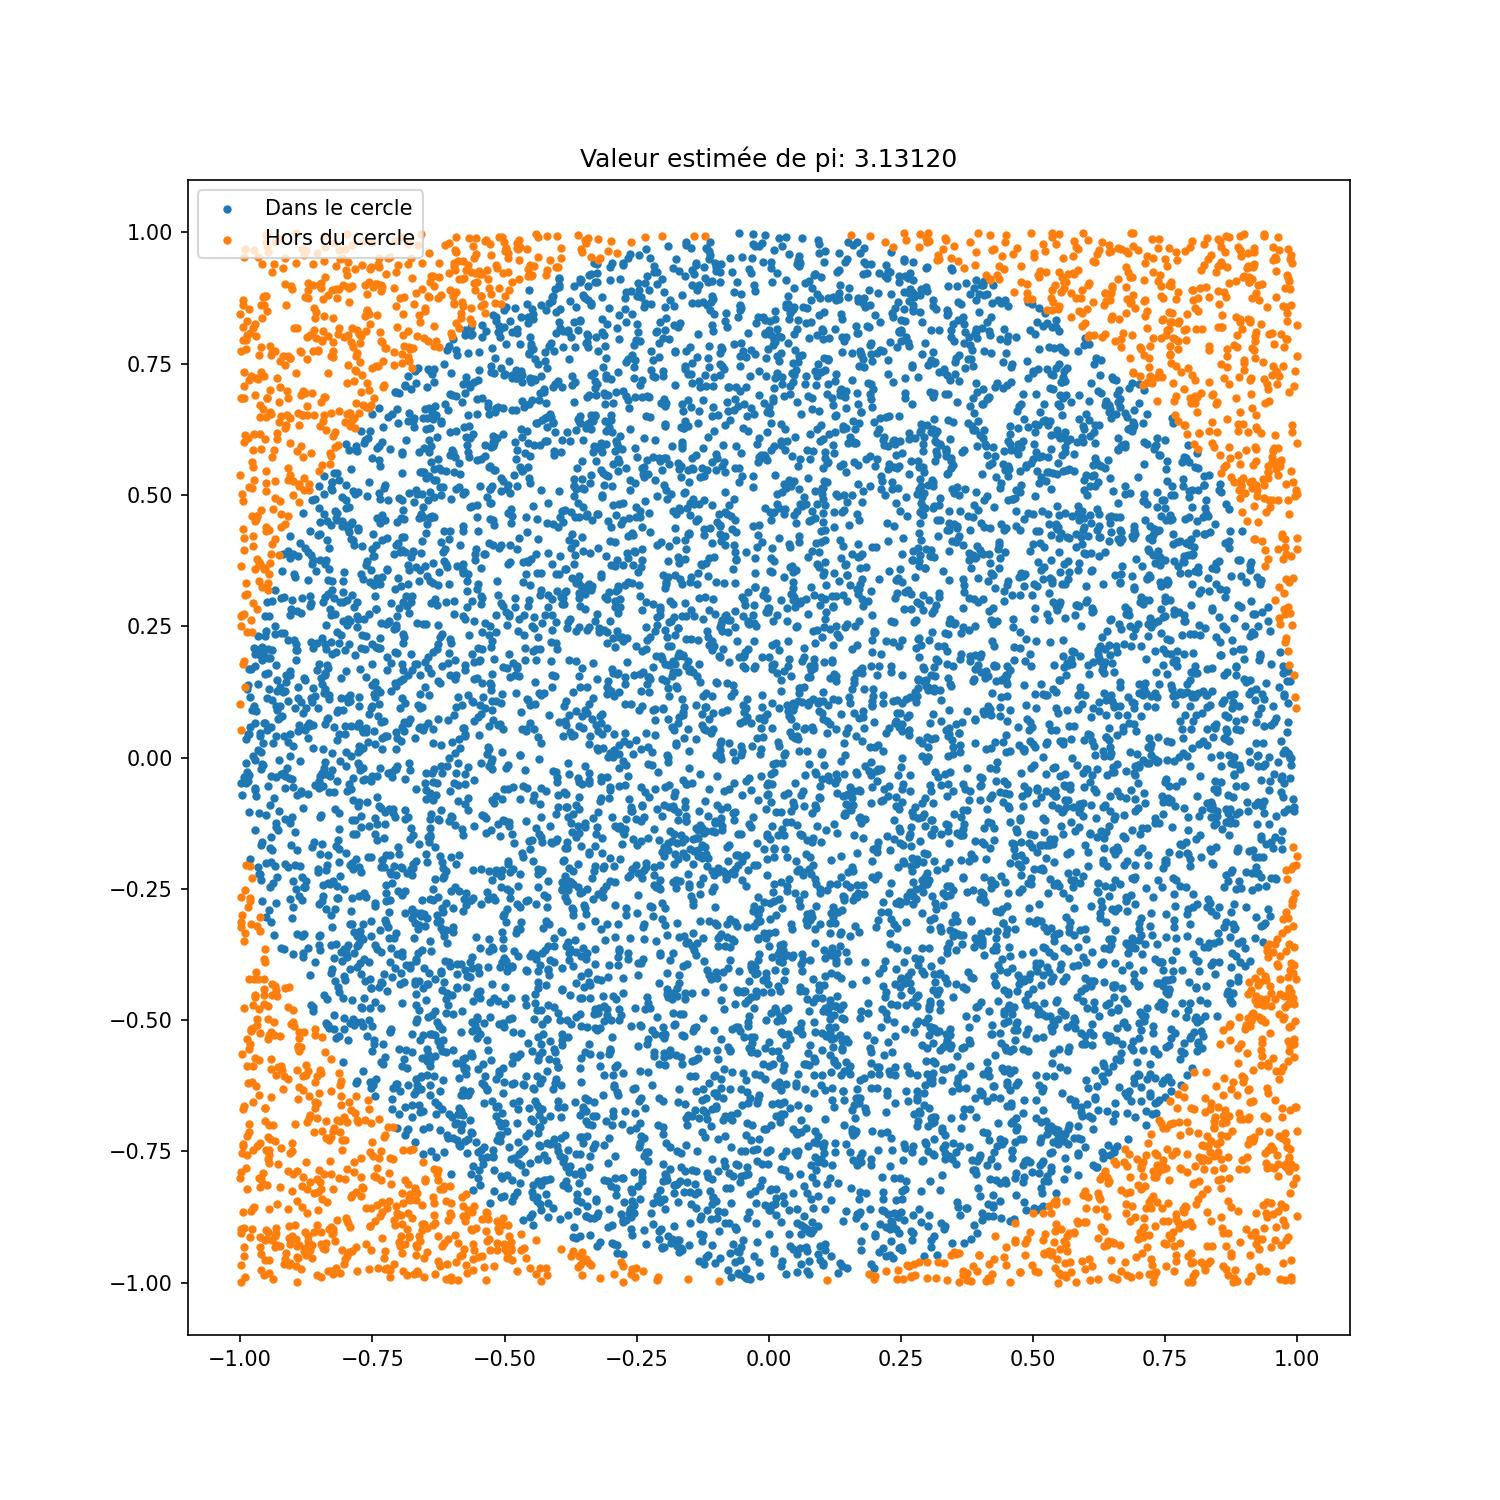
\includegraphics[width=0.7\textwidth]{images/montecarlo_pi.jpg}
                    \caption{Simulation Monte Carlo pour estimer la valeur de $\pi$}
                    \label{fig:montecarlo_pi}
                \end{figure}

        \subsubsection{Exercice 2: Estimation d'un point d'équilibre}
            Étant donné le système suivant:
            \begin{equation*}
                \begin{cases}
                    \dot{x}_1(t) = x_2(t)\\
                    \dot{x}_2(t) = -x_1(t) - x_2(t)
                \end{cases}
            \end{equation*}
            Étudiez, par Monte Carlo, la position du point d'équilibre du système. Pour ce faire, indiquez la position moyenne et la variance de la position après un temps arbitraire d'une grande quantité de conditions initiales aléatoires.
            
            La solution est donnée par le code suivant.
            \inputminted{python}{codes/montecarlo_point_d_equilibre.py}

        \subsubsection{Exercice 3: Estimation de la probabilité d'une position}
            Étant donné le système suivant:
            \begin{equation*}
                \begin{cases}
                    \dot{x}_1(t) = -x_2(t)\\
                    \dot{x}_2(t) = -x_1(t)
                \end{cases}
            \end{equation*}
            Soit un ensemble de conditions initiales $(x_1(0), x_2(0))$. 
            Étudiez, par Monte Carlo, après un temps arbitraire, la probabilité que la particule s'éloigne du cercle de rayon $x_1(0)^2 + x_2(0)^2$ d'au plus $10^{-3}$. Comment pouvez-vous expliquer le résultat grâce au portrait de phases de ce système ?
            
            La solution est donnée par le code suivant.
            \inputminted{python}{codes/montecarlo_trajectoires_cercle.py}

            Changez le seuil de tolérance pour $10^{-9}$. Les résultats tiennent-ils toujours? Pourquoi?